% Homework 22.tex 

\documentclass{article}
\usepackage{graphicx} % for figures
\usepackage{float}
\usepackage[export]{adjustbox}
\usepackage{fancyhdr}
\begin{document}

\title{Homework 22 - Physics 240\\
		Romberg integration}
\author{Tin Tran}

\maketitle

\section{Introduction}
The goal of this homework is to numerical integration to evaulate an integral. In this homework we use the Romberg integration

\section{Discussion and answer}
Originally the code provided didn't work for me, since the hstack and vstack ran into the issue of the array not being the same size, and I could not understand the logic of doing hstack after the vstack. So I modified the code to run a specific number of steps instead, then compute the error relative to the tolerance indepedently. So for the function I = $\frac{2}{\sqrt{\pi}}\int_0^1e^{-x^2}dx$, the answer I got with 14 iterations is 0.84270079 and the error is 2.29380266458e-10 \\
The full Romberg table can be seen when run the program, note that the process takes quite a bit of time(approximately 1 minute or more) when the number of steps is more than 22. I could not get the values to be on a diagonal, it could because I did not stack them properly. When I have the time I would fix that, but I can't do that now\\
Compared to the numpy.romberg() function, which gives the answer of 0.84270079295 after 33 interations, I say my code is pretty good for the tolerance value and and the error it gives.

\section{}
a) Values 1.93887342
\begin{figure}[H]
\centering{
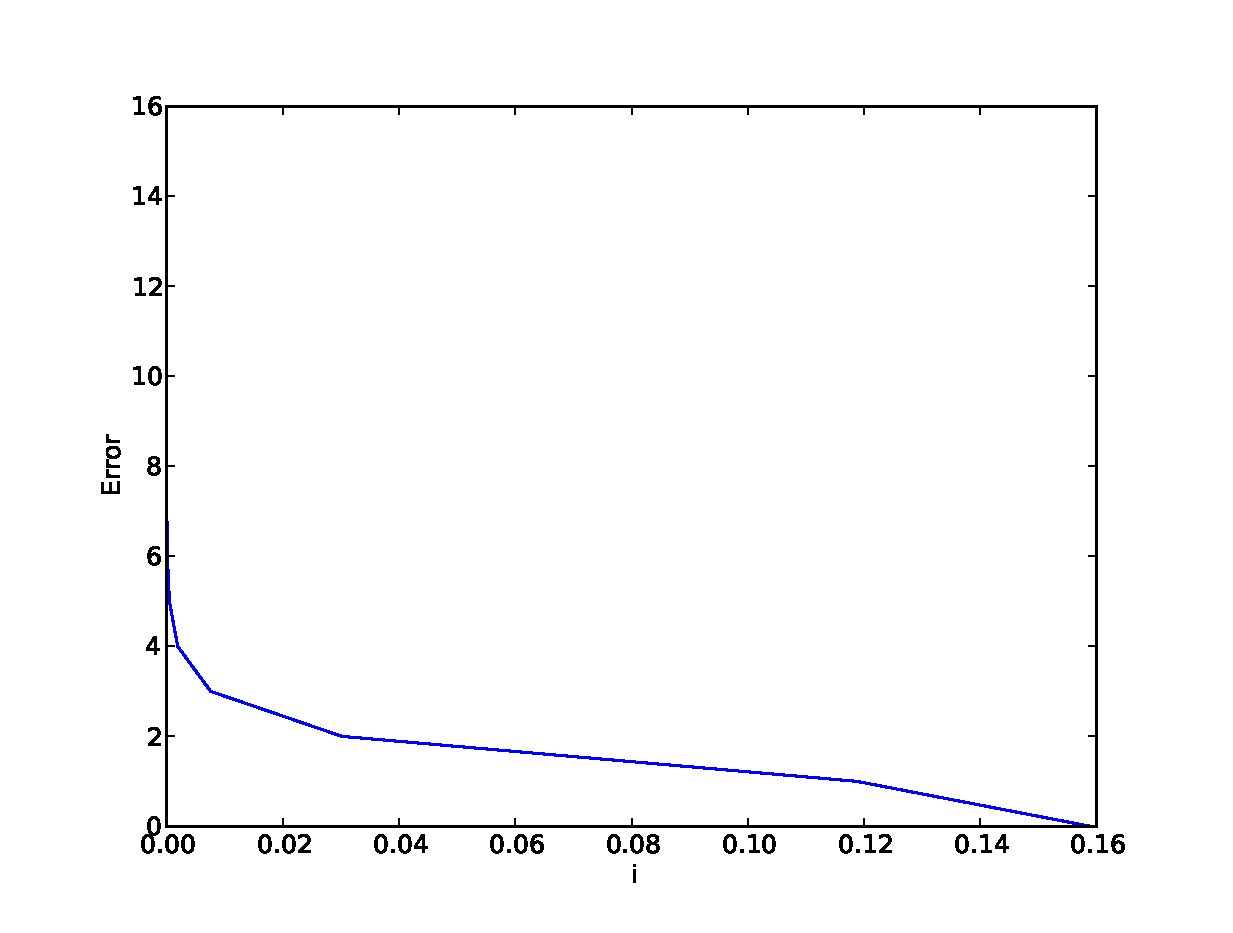
\includegraphics[max size={3 in}{4 in}]{hw22a.eps}
\caption{$\int_0^1e^{-x^2}dx$}
}
\end{figure}
b) Value: 2.65868078e+00
\begin{figure}[H]
\centering{
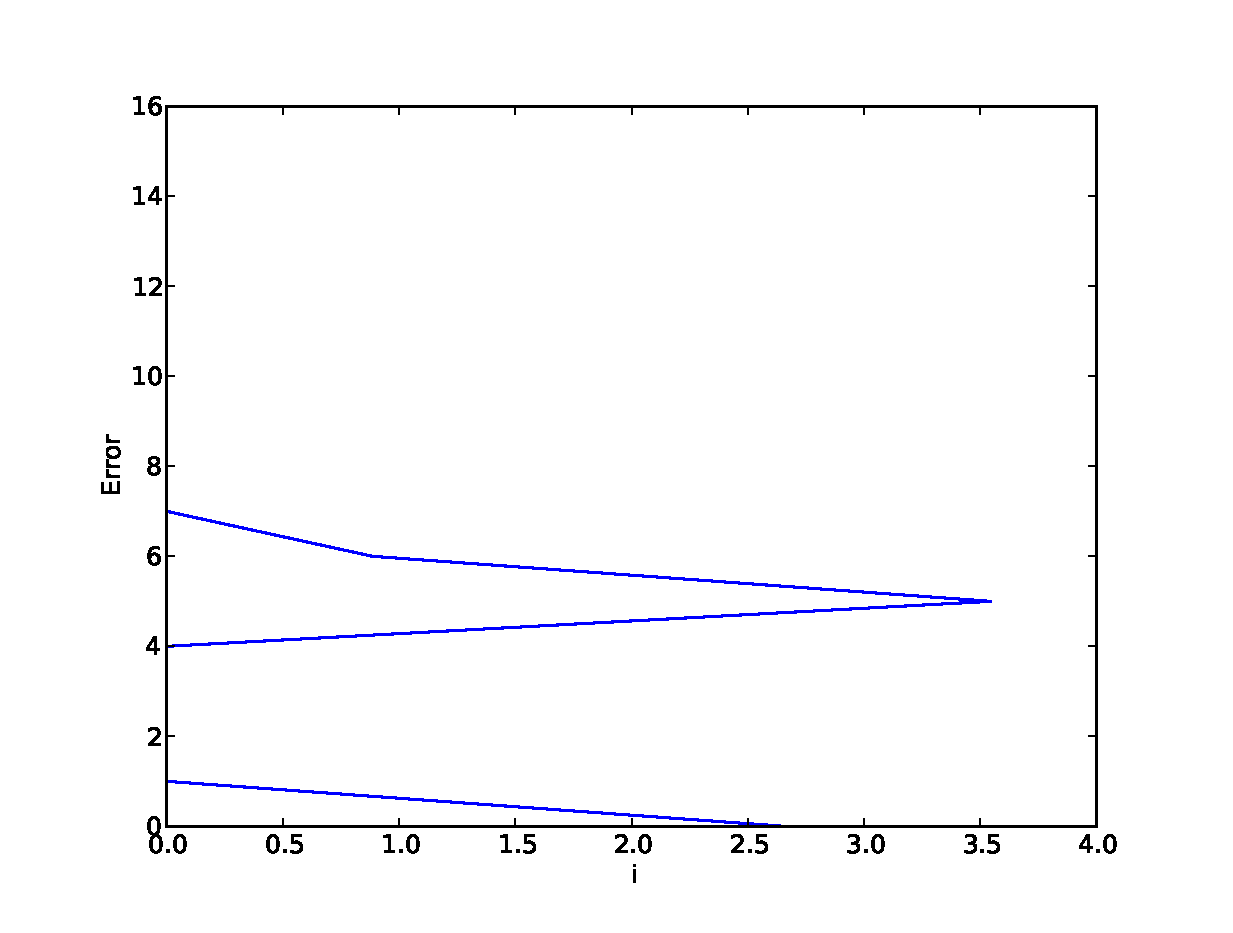
\includegraphics[max size={3 in}{4 in}]{hw22b.eps}
\caption{$\int_0^{2\pi}sin^4(8x)dx$}
}
\end{figure}
c) Value: 0.75225274
\begin{figure}[H]
\centering{
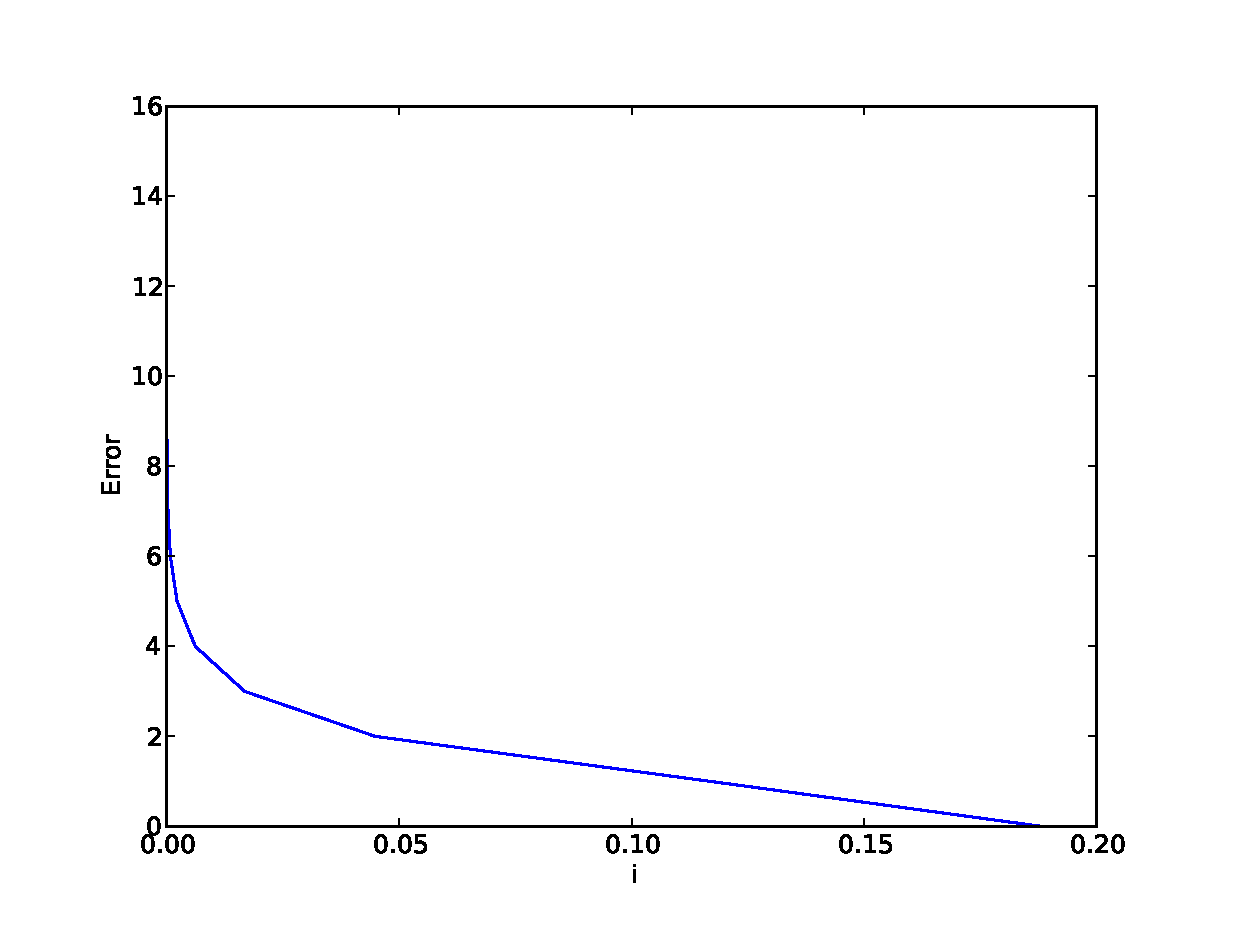
\includegraphics[max size={3 in}{4 in}]{hw22c.eps}
\caption{$\int_0^{1}\sqrt xdx$}
}
\end{figure}

d) Value: 0.88622687
\begin{figure}[H]
\centering{
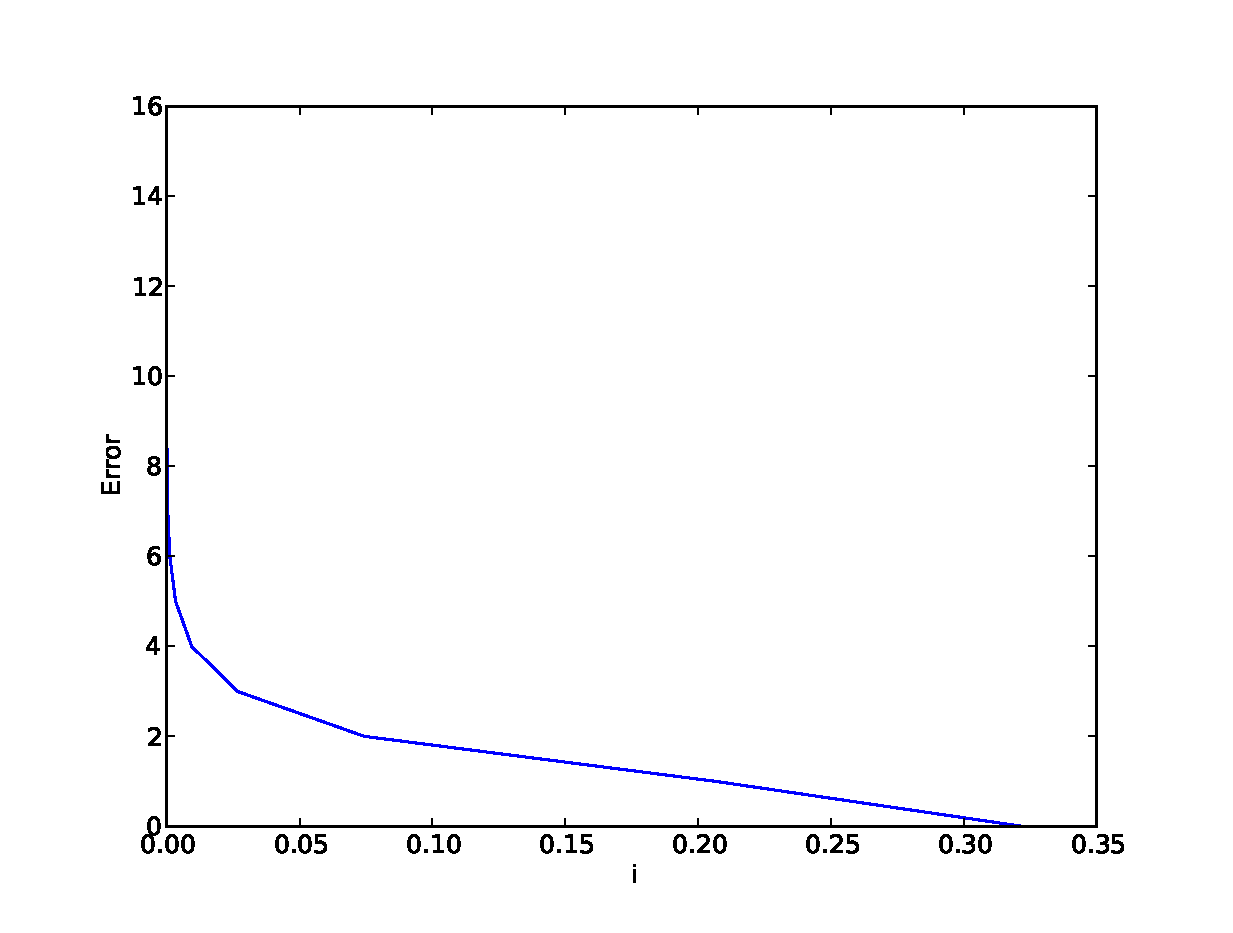
\includegraphics[max size={3 in}{4 in}]{hw22d.eps}
\caption{$\int_0^{1}\sqrt xdx$}
}
\end{figure}
e) Value: 0\\
f) Value: I don't know how to put this into Python\\
** Because of time constrain I could not figure out the stacking to make the Romberg table to look nicer. I will work on it when I have time.
\end{document}